% Created 2017-03-02 Thu 16:19
% Intended LaTeX compiler: pdflatex
\documentclass[10pt,aspectratio=1610]{beamer}
\usepackage[utf8]{inputenc}
\usepackage[T1]{fontenc}
\usepackage{graphicx}
\usepackage{grffile}
\usepackage{longtable}
\usepackage{wrapfig}
\usepackage{rotating}
\usepackage[normalem]{ulem}
\usepackage{amsmath}
\usepackage{textcomp}
\usepackage{amssymb}
\usepackage{capt-of}
\usepackage{hyperref}
\usepackage[english]{babel}\usepackage{etex}\usepackage{minted}\usemintedstyle{emacs}
\usepackage{tikz}\usepackage{amsmath}\usepackage[T1]{fontenc}\usepackage{lmodern}%\usepackage{arev}
\usepackage{booktabs}\usepackage[citestyle=alphabetic,bibstyle=authortitle]{biblatex}
\usepackage{pgfplots,pgfplotstable}\usetikzlibrary{pgfplots.groupplots}\usepackage[babel=true,kerning=true]{microtype}\usepackage{smartdiagram}
\addbibresource{fe.bib}
\usetikzlibrary{mindmap,trees,shapes,arrows,spy,3d,decorations.pathmorphing,pgfplots.statistics,pgfplots.dateplot}
\usetheme{DarkConsole}
\author{Mathieu Fauvel}
\date{\textit{[2017-04-26 Wed 10:30]--[2017-04-26 Wed 12:00]}}
\title{Feature Extraction}
\subtitle{GRSS Summer School}
\institute{UMR Dynafor}
\AtBeginSection[]{\begin{frame}<beamer>\frametitle{Outline}\tableofcontents[currentsection]\end{frame}}
\AtBeginSubsection[]{\begin{frame}<beamer>\frametitle{Outline}\tableofcontents[currentsubsection]\end{frame}}
\setbeamercovered{again covered={\opaqueness<1->{25}}}
\usefonttheme[onlymath]{serif}
\begin{document}

\maketitle
\begin{frame}{Outline}
\tableofcontents
\end{frame}


\section{Motivations}
\label{sec:org34ae4b3}
\begin{frame}[label={sec:org4136f0b}]{Illustration}
\begin{itemize}
\item <1-> \alert{Curse of dimensionality}: it is not possible to get enough data to cover all the observation space.
\begin{center}
\emph{High dimensional saces are mostly empty !}
\end{center}
\item <2> Multivariate data live in a lower dimensional space
\begin{center}
  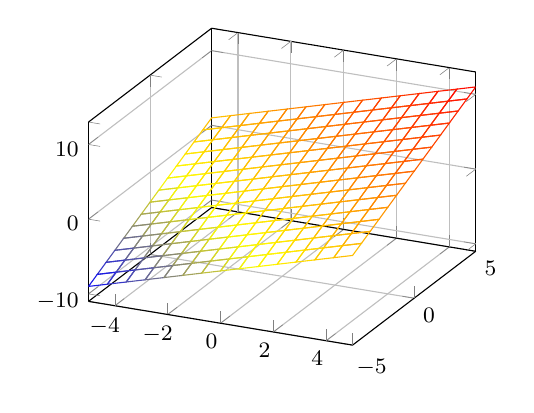
\begin{tikzpicture}
    \begin{axis}[grid=major,small]
      \addplot3 [mesh, samples=15, domain=-5:5] {x+y+1};
    \end{axis}
  \end{tikzpicture}
\end{center}
\end{itemize}
\end{frame}
\begin{frame}[label={sec:org5670ac8}]{Application}
\begin{itemize}
\item Feature extraction is important in remote sensing because:
\begin{itemize}
\item It reduces the size of the data,
\item It limits the spatial and spectral redundancy,
\item It permits visualization of the data,
\item It mitigates the \emph{curse of dimensionality}.
\end{itemize}
\item Extraction techniques:
\begin{itemize}
\item Spectral
\begin{itemize}
\item Physically based method,
\item Statistical methods.
\end{itemize}
\item Spatial:
\begin{itemize}
\item Linear filters,
\item Non linear techniques (Mathematical Morphology)
\end{itemize}
\end{itemize}
\end{itemize}
\end{frame}


\section{Physical Indices}
\label{sec:org76a5b97}
\subsection{Introduction}
\label{sec:org479da86}
\begin{frame}[label={sec:org4eb7e31}]{Spectral indices}
\begin{itemize}
\item Spectral indices are a linear/non-linear combination of two (or more) spectral bands.
\item They provides information as a \emph{single number} about:
\begin{itemize}
\item Plant structure,
\item Biochemistry,
\item Humidity,
\item Stress.
\end{itemize}
\item Four main types \cite{hrsv:2011}:
\begin{center}
\begin{tabular}{ll}
\toprule
Name & Formulae\\
\midrule
Difference vegetation index & \(R_{\lambda_1} - R_{\lambda_2}\)\\
Ratio vegetation index & \(\dfrac{R_{\lambda_1}}{R_{\lambda_2}}\)\\
Normalized difference vegetation index & \(\dfrac{R_{\lambda_1} - R_{\lambda_2}}{R_{\lambda_1} + R_{\lambda_2}}\)\\
Soil-adjusted vegetation index & \((1+L)\times\dfrac{R_{\lambda_1} - R_{\lambda_2}}{R_{\lambda_1} - R_{\lambda_2}+L}\)\\
\bottomrule
\end{tabular}
\end{center}
\item \emph{The three last indexes are invariant to  a multiplicative factor}
\end{itemize}
\end{frame}

\begin{frame}[label={sec:org7bb2ab1}]{Conventional Indices}
Index database : \url{http://www.indexdatabase.de/}

\begin{center}
\small
\begin{tabular}{ll}
\toprule
Name & Formulae  (\(\lambda\) nm)\\
\midrule
Normalized Difference Vnegetation index & \(\dfrac{R_{\lambda_{800}} - R_{\lambda_{670}}}{R_{\lambda_{800}} + R_{\lambda_{670}}}\)\\
Modified Soil-Adjusted Vegetation Index & \(\dfrac{1}{2}\left[2R_{\lambda_{800}}+1 - \sqrt{(2R_{\lambda_{800}}+1)^2-8(R_{\lambda_{800}}-R_{\lambda_{670}})}\right]\)\\
Modified Chlorophyll Absorption Ratio Index & \(\left[(R_{\lambda_{700}}-R_{\lambda_{670}})-0.2(R_{\lambda_{700}}-R_{\lambda_{550}})\right]\times\dfrac{R_{\lambda_{700}}}{R_{\lambda_{670}}}\)\\
\midrule
Normalized Difference Water Index & \(\dfrac{R_{\lambda_{858}} - R_{\lambda_{1240}}}{R_{\lambda_{858}} + R_{\lambda_{1240}}}\)\\
Datt Reflectance Index & \(\dfrac{R_{\lambda_{816}} - R_{\lambda_{2218}}}{R_{\lambda_{816}} + R_{\lambda_{2218}}}\)\\
\midrule
Normalized Difference Redness Index & \(\dfrac{R_{\lambda_{540}} - R_{\lambda_{700}}}{R_{\lambda_{540}} + R_{\lambda_{700}}}\)\\
Soil Brightness Index & \(0.406R_{\lambda{550}}+0.600R_{\lambda{650}}+0.645R_{\lambda{750}}+0.243R_{\lambda{950}}\)\\
\bottomrule
\end{tabular}
\end{center}
\end{frame}

\subsection{Vegetation Indices}
\label{sec:org76971da}
\begin{frame}[label={sec:orgeb5e234}]{Normalized difference vegetation index}
$$\text{NDVI}=\dfrac{R_{\lambda_{800}} - R_{\lambda_{670}}}{R_{\lambda_{800}} + R_{\lambda_{670}}}$$
\begin{itemize}
\item \(-1\leq \text{NVDI} \leq 1\)
\item \(\text{NDVI}< 0\): surfaces other thatn plant cover
\item \(\text{NDVI}\approx 0\): bare soil
\item \(\text{NDVI}\geq 0.1\): vegetation cover (higher values correspond to more dense covers)
\end{itemize}

\begin{center}
\begin{tikzpicture}
\begin{axis}[xmin=0.4,xmax=1,ymin=0,ymax=1,grid,xlabel=$\lambda~({\mu}m)$,ylabel=Reflectance,width=0.6\linewidth,height=0.3\linewidth,cycle list name=color list]
  \addplot+[mark=none,thick,smooth] file {../Introduction/figures/oak.txt};
  \pgfplotstableread{../Introduction/figures/grass.txt}\loadedtable
  \addplot+[mark=none,smooth,thick] table[x=wave,y=grass] from \loadedtable;
  \addplot+[mark=none,smooth,thick] table[x=wave,y=drygrass] from \loadedtable;
  \pgfplotstableread{../Introduction/figures/talc.txt}\loadtable
  \addplot+[mark=none,smooth,thick] table[x=wave,y=talc] from \loadtable;
  \legend{0.81,0.90, 0.05, -0.03}
\end{axis}
\end{tikzpicture}
\end{center}
\end{frame}
\begin{frame}[label={sec:orgc77bd24}]{Modified Soil-Adjusted Vegetation Index}
\end{frame}
\subsection{Case study}
\label{sec:orgefa969b}
\begin{frame}[label={sec:orgbdb3794}]{University of Pavia}
\begin{columns}
\begin{column}{0.5\columnwidth}
\begin{center}
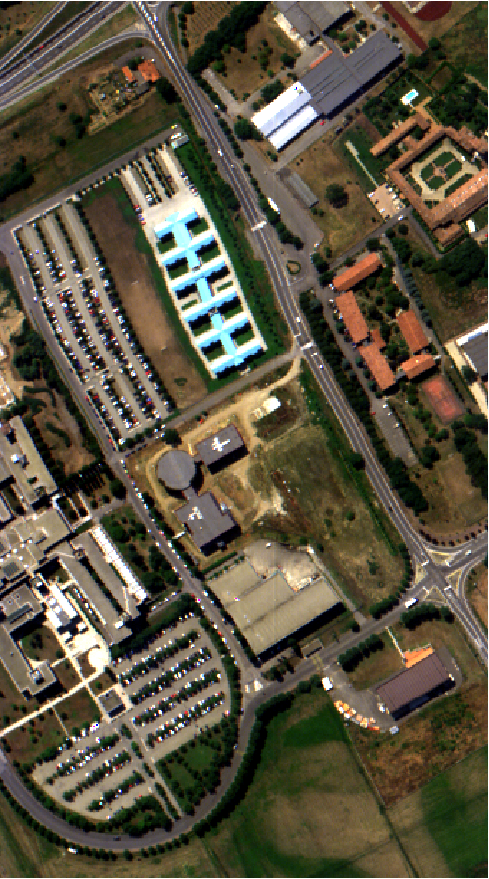
\includegraphics[width=0.6\linewidth]{./figures/university_color.png}
\end{center}
\end{column}

\begin{column}{0.5\columnwidth}
\begin{itemize}
\item Peri-urban area
\item Rosis-3 sensor
\item 103 Spectral bands (400nm-900nm)
\item 1.5 meter per pixel spatial resolution
\item 610 \(\times\) 340 pixels
\end{itemize}
\end{column}
\end{columns}
\end{frame}

\begin{frame}[fragile,label={sec:orge44d26d}]{Orfeo-Toolbox}
 \begin{itemize}
\item \href{https://www.orfeo-toolbox.org/}{OTB} is a C++ library for remote sensing images processing.
\item It is free, open-source and available for most OS (window, apple, linux)
\item \href{https://www.orfeo-toolbox.org/CookBook/OTB-Applications.html}{OTB-Applications} are set of tools appropriated for big/large images
\item They are avalaible from QGIS, Python and Bash
\item To compute the NDVI
\end{itemize}

\begin{minted}[fontsize=\footnotesize,obeytabs=true,tabsize=4,bgcolor=bg]{bash}
# Computation of the NDVI
otbcli_BandMath -il ../Data/university.tif -out ../Data/university_ndvi.tif \
		-exp "(im1b83-im1b56)/(im1b83+im1b56)"

# Computation of the SBI
otbcli_BandMath -il ../Data/university.tif -out ../Data/university_sbi.tif \
		-exp "0.406*im1b31 + 0.6*im1b52 + 0.645*im1b73"
\end{minted}
\end{frame}

\begin{frame}[label={sec:org69da580}]{University of Pavia - Spectral Indices}
\begin{columns}
\begin{column}{0.3\columnwidth}
\begin{center}
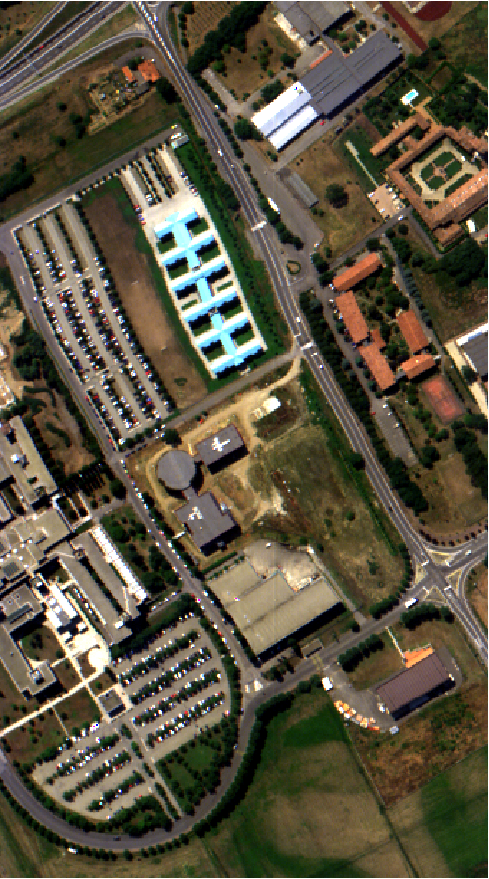
\includegraphics[width=\linewidth]{./figures/university_color.png}
\end{center}
\end{column}

\begin{column}{0.3\columnwidth}
\begin{center}
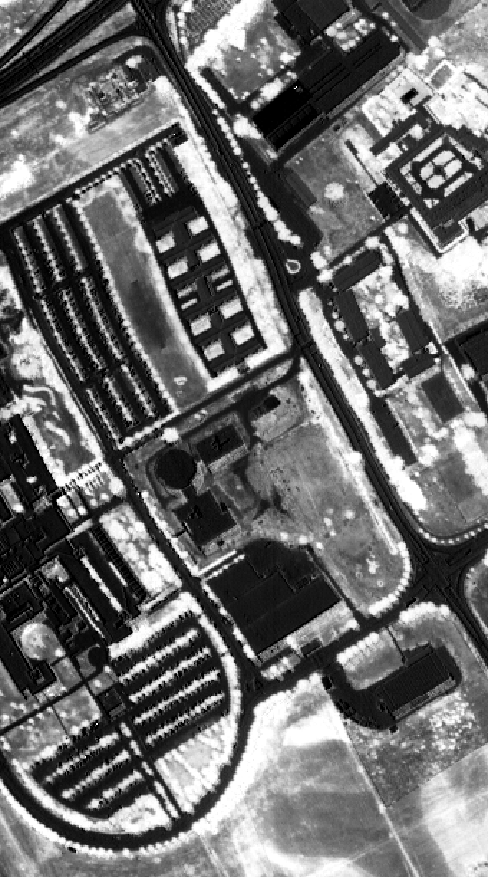
\includegraphics[width=\linewidth]{./figures/university_ndvi.png}
\end{center}
\end{column}

\begin{column}{0.3\columnwidth}
\begin{center}
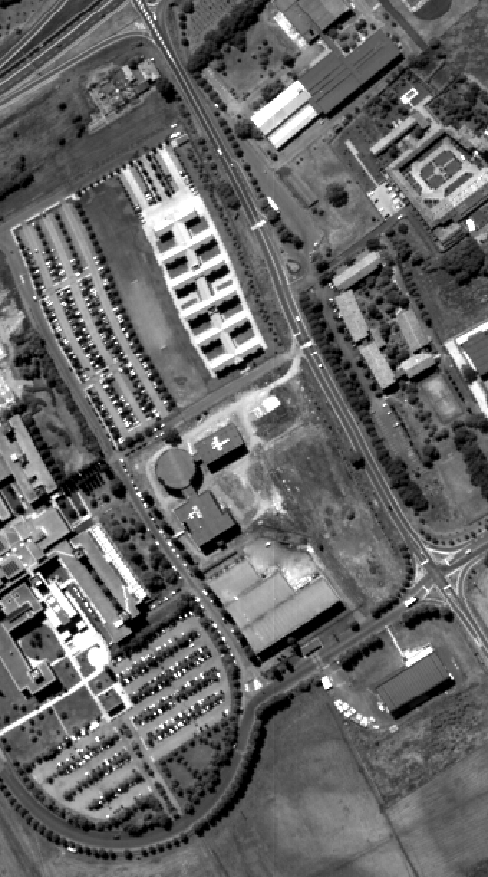
\includegraphics[width=\linewidth]{./figures/university_sbi.png}
\end{center}
\end{column}
\end{columns}
\end{frame}

\begin{frame}[fragile,label={sec:org785e1bf}]{Where is the vegetation 1/2 ?}
   \begin{center}
  \begin{tikzpicture}
    \begin{axis}[grid=both,width=0.95\linewidth,height=0.45\linewidth,/pgf/number format/1000 sep={},/pgf/number format/fixed,title=Histogram of the NDVI,xmin=-0.6,xmax=1]
      \addplot+[mark=none,thick,smooth] table[x=x,y=y,col sep=comma] {figures/pdf.csv};
      \only<2->{\addplot[red,thick] coordinates {(0.19,0) (0.19,0.008)};
      \addplot[red,thick] coordinates {(0.62,0) (0.62,0.008)}; }     
    \end{axis}
\end{tikzpicture}
\end{center}

\begin{minted}[fontsize=\footnotesize,obeytabs=true,tabsize=4,bgcolor=bg]{bash}
# Segmentation of the NDVI in three classes
otbcli_BandMath -il ../Data/university_ndvi.tif -out ../Data/university_ndvi_segmented.tif \
		-exp "(im1b1<0.19?1:(im1b1<0.62?2:3))"
\end{minted}
\end{frame}

\begin{frame}[label={sec:org986c9db}]{Where is the vegetation 2/2 ?}
\begin{columns}
\begin{column}{0.5\columnwidth}
\begin{center}
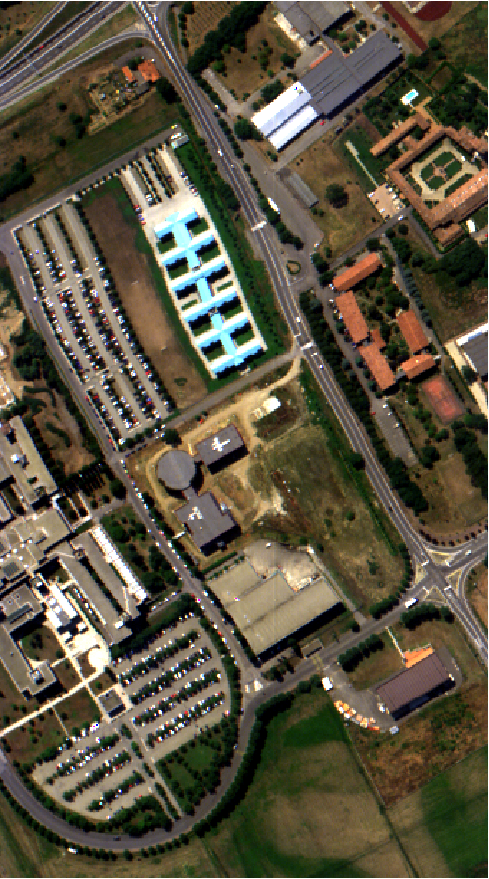
\includegraphics[width=0.6\linewidth]{./figures/university_color.png}
\end{center}
\end{column}

\begin{column}{0.5\columnwidth}
\begin{center}
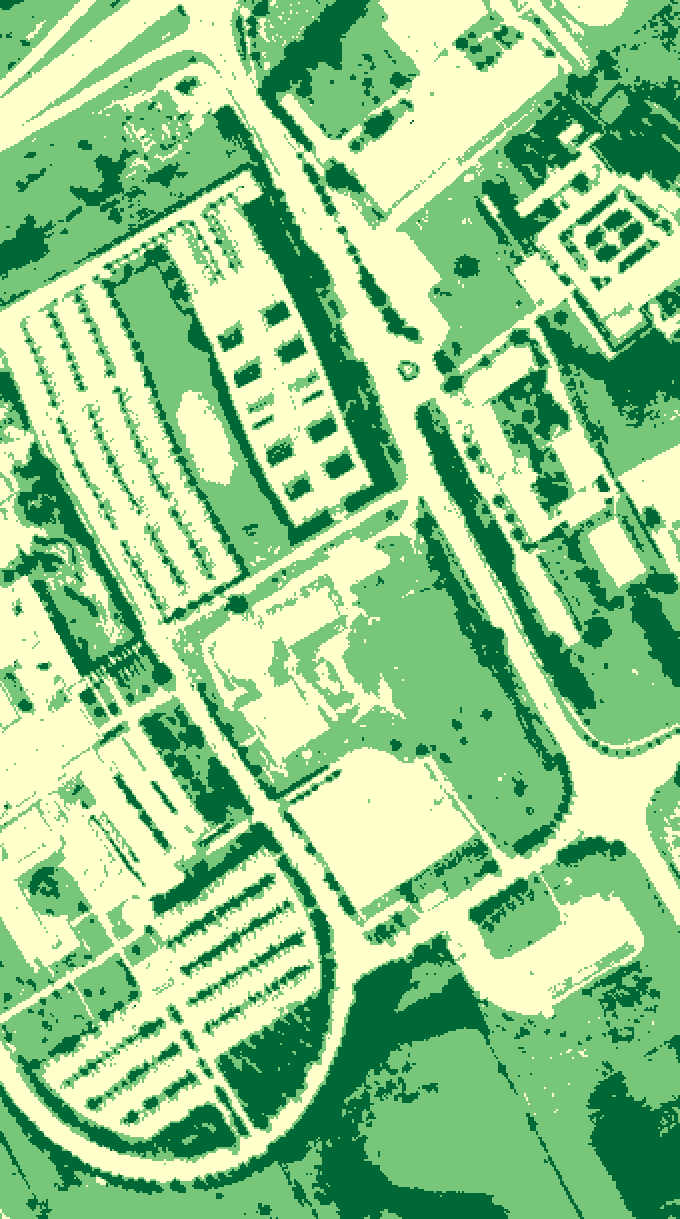
\includegraphics[width=0.6\linewidth]{./figures/university_ndvi_segmented.png}
\end{center}
\end{column}
\end{columns}
\end{frame}

\subsection{Question}
\label{sec:org03e7bd6}
\begin{frame}[label={sec:orgf23d211}]{Could you find the good one ?}
 \centerline{\begin{tabular}{cc}
    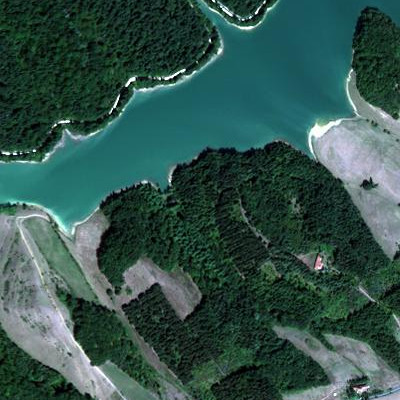
\includegraphics[width=0.4\linewidth]{figures/image1.jpg} & \begin{tikzpicture}\pgfplotsset{every axis legend/.append style={at={(0.5,1.03)},anchor=south}}
      \begin{axis}[ytick=\empty,xmin=-0.5,xmax=0.9,ymin=0,width=0.5\linewidth,axis y line=center,axis x line=bottom,legend columns=4]
        \pgfplotstableread{figures/ndvi1.txt}\loadedtable
        \addplot[smooth,very thick,dashed,blue] table[x=wave,y=ndvi] from \loadedtable;
        \pgfplotstableread{figures/ndvi2.txt}\loadedtable
        \addplot[smooth,very thick,magenta] table[x=wave,y=ndvi] from \loadedtable;
        \pgfplotstableread{figures/ndvi3.txt}\loadedtable
        \addplot[smooth,very thick,dotted,orange] table[x=wave,y=ndvi] from \loadedtable;
        \pgfplotstableread{figures/ndvi4.txt}\loadedtable
        \addplot[smooth,very thick,dashdotted,green] table[x=wave,y=ndvi] from \loadedtable;
        \legend{ndvi$_1$,ndvi$_2$,ndvi$_3$,ndvi$_4$};
      \end{axis}
    \end{tikzpicture}\\
    Image & NDVI Histogram
\end{tabular}}

From the histogram, which one does correspond to the NDVI of the image ?
\end{frame}
\section{Statistical Feature Extraction}
\label{sec:orgfc9c661}

\subsection{Unsupervised}
\label{sec:org6db8f84}

\subsection{Supervised}
\label{sec:org812a1cd}

\section{Spatial feature extaction}
\label{sec:orgbbd3772}

\subsection{Linear filters}
\label{sec:orgc47f32e}

\subsection{Mathematical morphology}
\label{sec:org5af4d09}
\end{document}